% Original vector drawings. The three isometric unit vectors project to zero in sum.
\definecolor{boxink}{HTML}{223A41}
\definecolor{boxtop}{HTML}{F2D5A3}
\definecolor{boxleft}{HTML}{96BDB5}
\definecolor{boxright}{HTML}{5D9196}
\definecolor{boxgrid}{HTML}{B5C2C1}
\definecolor{boxwarm}{HTML}{E5B977}
\tikzset{boxface/.style={draw=boxink,line width=.46pt,line join=round}}

\newcommand{\TopTile}[3]{\filldraw[boxface,fill=boxtop]
  (#1,#2,#3) -- ++(1,0,0) -- ++(0,1,0) -- ++(-1,0,0) -- cycle;}
\newcommand{\XTile}[3]{\filldraw[boxface,fill=boxright]
  (#1,#2,#3) -- ++(0,1,0) -- ++(0,0,1) -- ++(0,-1,0) -- cycle;}
\newcommand{\YTile}[3]{\filldraw[boxface,fill=boxleft]
  (#1,#2,#3) -- ++(1,0,0) -- ++(0,0,1) -- ++(-1,0,0) -- cycle;}
\newcommand{\BoxOutline}{(0,0,4) -- (2,0,4) -- (2,0,0) --
  (2,2,0) -- (0,2,0) -- (0,2,4) -- cycle}

% Heights by row are (4,2) and (1,0).
\newcommand{\SevenCubes}{%
  \TopTile{0}{0}{4}\TopTile{1}{0}{2}\TopTile{0}{1}{1}
  \foreach \x/\y/\z in {2/0/0,2/0/1,1/0/2,1/0/3,1/1/0}{\XTile{\x}{\y}{\z}}
  \foreach \x/\y/\z in {0/2/0,0/1/1,0/1/2,0/1/3,1/1/0,1/1/1}{\YTile{\x}{\y}{\z}}}
\newcommand{\EmptyCornerFaces}{%
  \begingroup
  \colorlet{boxtop}{boxtop!20!white}
  \colorlet{boxleft}{boxleft!37!white}
  \colorlet{boxright}{boxright!37!white}
  \TopTile{1}{1}{0}
  \foreach \z in {1,2,3}{\XTile{0}{1}{\z}}
  \foreach \z in {2,3}{\YTile{1}{0}{\z}}
  \endgroup}

\newcommand{\StackAndTiling}{%
  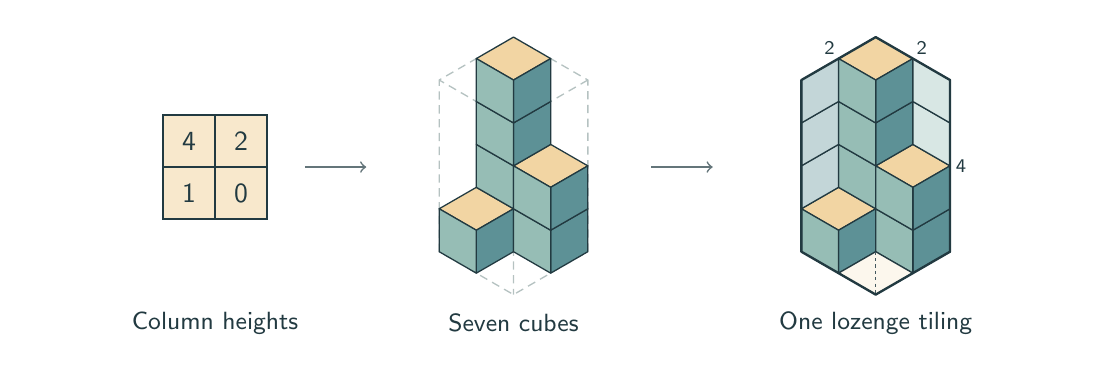
\begin{tikzpicture}[font=\sffamily\small,text=boxink]
    \path[use as bounding box] (-.12,-1.40) rectangle (13.05,2.52);
    \begin{scope}[shift={(1.60,.75)},x=.66cm,y=.66cm]
      \foreach \x/\y/\n in {0/0/4,1/0/2,0/-1/1,1/-1/0}{
        \draw[boxink,fill=boxtop!55,line width=.5pt] (\x,\y) rectangle ++(1,1);
        \node[font=\sffamily\normalsize] at ({\x+.5},{\y+.5}) {\n};}
    \end{scope}
    \draw[->,draw=boxink!70,line width=.6pt] (3.40,.75)--(4.18,.75);
    \begin{scope}[shift={(6.05,.22)},x={(.472cm,-.2725cm)},
                            y={(-.472cm,-.2725cm)},z={(0cm,.545cm)}]
      \draw[boxgrid,densely dashed,line width=.48pt] \BoxOutline;
      \draw[boxgrid,densely dashed,line width=.48pt]
        (2,0,0)--(0,0,0)--(0,2,0) (0,0,0)--(0,0,4)
        (2,0,4)--(2,2,4)--(0,2,4) (2,2,4)--(2,2,0);
      \SevenCubes
    \end{scope}
    \draw[->,draw=boxink!70,line width=.6pt] (7.80,.75)--(8.58,.75);
    \begin{scope}[shift={(10.65,.22)},x={(.472cm,-.2725cm)},
                            y={(-.472cm,-.2725cm)},z={(0cm,.545cm)}]
      \SevenCubes\EmptyCornerFaces
      \draw[draw=boxink!85,dash pattern=on 1.2pt off 1.1pt,line width=.42pt]
        (1,1,0)--(2,2,0);
      \draw[boxink,line width=.85pt,line join=round] \BoxOutline;
      \path (0,2,4)--(0,0,4) node[midway,above left,inner sep=1.2pt,font=\sffamily\scriptsize] {2};
      \path (0,0,4)--(2,0,4) node[midway,above right,inner sep=1.2pt,font=\sffamily\scriptsize] {2};
      \path (2,0,4)--(2,0,0) node[midway,right,inner sep=1.9pt,font=\sffamily\scriptsize] {4};
    \end{scope}
    \node at (2.26,-1.23) {Column heights};
    \node at (6.05,-1.23) {Seven cubes};
    \node at (10.65,-1.23) {One lozenge tiling};
  \end{tikzpicture}}

% One projected square. The angle is the first of its three rim vertices.
\newcommand{\UnitFaceInTiling}[2]{%
  \filldraw[draw=boxink,fill=#2,line width=.78pt]
    (0,0)--(#1:1)--({#1+60}:1)--({#1+120}:1)--cycle;
  \draw[draw=boxink!74,line width=.50pt,densely dotted]
    (0,0)--({#1+60}:1);}

% Left column: oblique physical views with the vertical axis upright.
% Right column: Figure 1's diagonal projection turned counterclockwise 90
% degrees. From the empty back corner the x,y,z rays have angles 60,300,180.
% The exposed edges at the opposite corner of the cube use the reverse rays.
\newcommand{\TwoUnitTilings}{%
  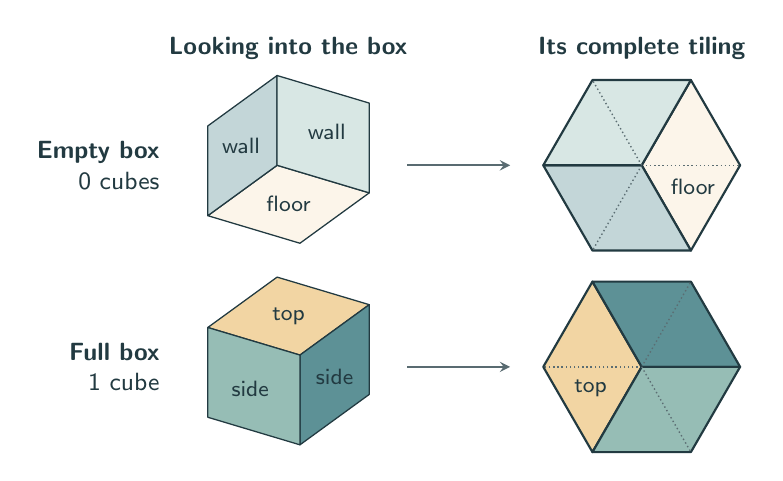
\begin{tikzpicture}[text=boxink,font=\sffamily\small,line join=round,>=stealth]
    \node[font=\sffamily\small\bfseries] at (.14,1.49) {Looking into the box};
    \node[font=\sffamily\small\bfseries] at (4.63,1.49) {Its complete tiling};
    \foreach \level/\offset/\stackname/\cubecount in
        {0/0/Empty box/0 cubes,1/-2.56/Full box/1 cube}{%
      \begin{scope}[shift={(0,\offset)}]
        \node[anchor=east,align=right] at (-1.37,0)
          {\textbf{\stackname}\\\cubecount};
        \begin{scope}[x={(1.17cm,-.35cm)},y={(-.88cm,-.64cm)},z={(0cm,1.14cm)},
            font=\sffamily\footnotesize]
          \ifnum\level=0\relax
            \colorlet{boxtop}{boxtop!23!white}
            \colorlet{boxleft}{boxleft!37!white}
            \colorlet{boxright}{boxright!37!white}
            \TopTile{0}{0}{0}\XTile{0}{0}{0}\YTile{0}{0}{0}
            \node at (.5,.5,0) {floor};
            \node at (0,.52,.51) {wall};
            \node at (.54,0,.54) {wall};
          \else
            \TopTile{0}{0}{1}\XTile{1}{0}{0}\YTile{0}{1}{0}
            \node at (.5,.5,1) {top};
            \node at (1,.50,.48) {side};
            \node at (.46,1,.46) {side};
          \fi
        \end{scope}
        \draw[->,draw=boxink!75,line width=.64pt] (1.65,0)--(2.96,0);
        \begin{scope}[shift={(4.63,0)},scale=1.25,font=\sffamily\footnotesize]
          \ifnum\level=0\relax
            \UnitFaceInTiling{300}{boxtop!23!white}
            \UnitFaceInTiling{180}{boxright!37!white}
            \UnitFaceInTiling{60}{boxleft!37!white}
            \node at (.52,-.22) {floor};
          \else
            \UnitFaceInTiling{120}{boxtop}
            \UnitFaceInTiling{0}{boxright}
            \UnitFaceInTiling{240}{boxleft}
            \node at (-.52,-.22) {top};
          \fi
        \end{scope}
      \end{scope}}
  \end{tikzpicture}}

% Before and after the same move on a unit hexagon. Only the two upward
% triangles sharing an edge with the dotted triangle receive an increment.
\newcommand{\LabelBoards}{%
  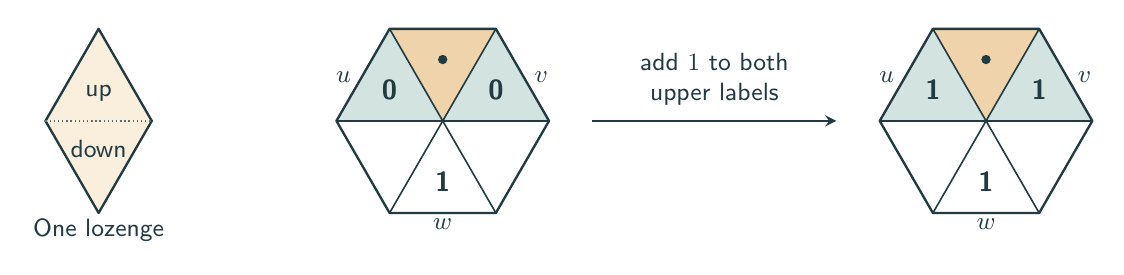
\begin{tikzpicture}[text=boxink,font=\sffamily\small,line join=round,>=stealth]
    \begin{scope}[shift={(-7.82,0)},scale=1.35]
      \filldraw[fill=boxtop!38,draw=boxink,line width=.85pt]
        (-.5,0)--(0,.8660254)--(.5,0)--(0,-.8660254)--cycle;
      \draw[draw=boxink!74,line width=.50pt,densely dotted] (-.5,0)--(.5,0);
      \node at (0,.26) {up};
      \node at (0,-.26) {down};
    \end{scope}
    \node[anchor=north,inner sep=2pt] at (-7.82,-1.17) {One lozenge};
    \foreach \offset/\upperentry in {-3.45/0,3.45/1}{%
      \begin{scope}[shift={(\offset,0)},scale=1.35]
        \fill[boxwarm!62] (0,0)--(60:1)--(120:1)--cycle;
        \fill[boxleft!42] (0,0)--(120:1)--(180:1)--cycle;
        \fill[boxleft!42] (0,0)--(0:1)--(60:1)--cycle;
        \foreach \angle in {0,60,...,300}
          \draw[boxink,line width=.58pt] (0,0)--(\angle:1);
        \draw[boxink,line width=.85pt]
          (0:1)--(60:1)--(120:1)--(180:1)--(240:1)--(300:1)--cycle;
        \fill[boxink] (0,.57735) circle[radius=1.25pt];
        \node[font=\sffamily\normalsize\bfseries] at (-.5,.288675) {\upperentry};
        \node[font=\sffamily\normalsize\bfseries] at ( .5,.288675) {\upperentry};
        \node[font=\sffamily\normalsize\bfseries] at (0,-.57735) {1};
        \node[anchor=east,inner sep=1.5pt] at (-.82,.41) {\(u\)};
        \node[anchor=west,inner sep=1.5pt] at ( .82,.41) {\(v\)};
        \node[anchor=north,inner sep=2pt] at (0,-.8660254) {\(w\)};
      \end{scope}}
    \draw[->,boxink,line width=.8pt] (-1.55,0)--(1.55,0);
    \node[above=2pt,align=center] at (0,0) {add \(1\) to both\\upper labels};
  \end{tikzpicture}}

\newcommand{\DegreeRow}[1]{%
  \draw[boxgrid,line width=.5pt] (0,#1)--(5,#1);
  \foreach \n in {0,1,4,5}{
    \node[draw=boxink,fill=boxleft!47,circle,inner sep=0pt,
          minimum size=12.5pt,line width=.5pt] at (\n,#1) {\n};}
  \foreach \n in {2,3}{
    \node[draw=boxgrid,fill=white,text=boxink!75,circle,inner sep=0pt,
          minimum size=12.5pt,line width=.45pt] at (\n,#1) {\n};}}
\newcommand{\ResiduePairs}{%
  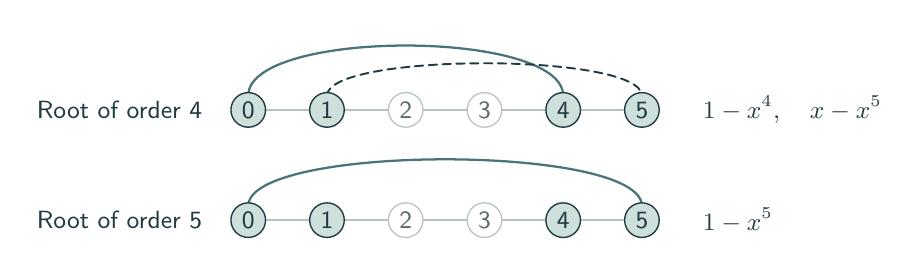
\begin{tikzpicture}[x=1.00cm,y=1cm,font=\sffamily\small,text=boxink,line cap=round]
    \node[anchor=east] at (-.46,1.35) {Root of order 4};
    \draw[boxright!80!black,line width=.82pt]
      (0,1.53) .. controls (0,2.38) and (4,2.38) .. (4,1.53);
    \draw[boxink,line width=.70pt,densely dashed]
      (1,1.53) .. controls (1,2.08) and (5,2.08) .. (5,1.53);
    \DegreeRow{1.35}
    \node[anchor=west] at (5.65,1.35) {\(\displaystyle 1-x^4,\quad x-x^5\)};
    \node[anchor=east] at (-.46,-.05) {Root of order 5};
    \draw[boxright!80!black,line width=.82pt]
      (0,.13) .. controls (0,.92) and (5,.92) .. (5,.13);
    \DegreeRow{-.05}
    \node[anchor=west] at (5.65,-.05) {\(\displaystyle 1-x^5\)};
  \end{tikzpicture}}
